\documentclass[a4paper]{article}
\usepackage{listings}
\usepackage{verbatim}
\usepackage{graphicx}
\usepackage{amsmath}
%% Language and font encodings
\usepackage[english]{babel}
\usepackage[utf8x]{inputenc}
\usepackage[T1]{fontenc}
\usepackage{csvsimple}
%% Sets page size and margins
\usepackage[a4paper,top=3cm,bottom=2cm,left=3cm,right=3cm,marginparwidth=1.75cm]{geometry}

%% Useful packages
\usepackage{amsmath}
\usepackage{graphicx}
\usepackage[colorinlistoftodos]{todonotes}
\usepackage[colorlinks=true, allcolors=blue]{hyperref}

\begin{document}
\begin{titlepage}
	\raggedleft
	\rule{1pt}{\textheight} 
	\hspace{0.05\textwidth} 
	\parbox[b]{0.75\textwidth}{		
		{\LARGE\bfseries EE - 2703 Applied Programming Lab \\[0.5\baselineskip]  ~\huge Assignment -5}\\[2\baselineskip] 
		{\large\textit{The Tube Light Model Simulation}}\\[4\baselineskip] 
		{\Large\textbf{Mohammed Khandwawala}}
        \large EE16B117
		\vspace{0.5\textheight}  
	}

\end{titlepage}


\tableofcontents


\section{Introduction}
This simulation consist of a 1 -D model of tubelight . In presence of an electric field the electron on the tube accelerates. Electrons are emitted from anode at rest and move towards cathode. In this model assumption is that after electron reaches critical energy it excites the atom ( of gas filed in the tube ) and comes to rest. Electrons reaching anode are lost. At every step new electrons are introduced in the tube . This number of new electron is given by normally distributed random number. And the process repeats.
Tube starts from x = 0 and ends at x = 100, where electron are absorbed in the anode.
\section{Parameters for the simulation}
The parameters are number of length of the tube(n), mean(M), number of iterations(nk), threshold or critical velocity(u0), probability of collision(p) and standard deviation(Msig).
All the inputs are given through command line . Default value of the arguments are already assigned.
\begin{lstlisting}[language=Python]

if(len(sys.argv) == 7):
	n = int(sys.argv[1])
	M = int(sys.argv[2])
	nk = int(sys.argv[3])
	u0 = float(sys.argv[4])
	p = float(sys.argv[5])
    Msig = float(sys.argv[6])
else:
	n=100 #spatial grid size
	M = 5 #number of electron injected per turn
	nk = 500 #number of turns to simulate
	u0 = 5 #threshold velocity
	p = 0.25 #probality that ionization will occur
	Msig = 2 #standard deviation of normal distribution


\end{lstlisting}


\section{Declaring vectors}
xx vector stores the position of the electrons in the tube . Similarly u stores velocity and dx displacement in current turn.
I,X and V are lists to store  intensity at all points , position and velocity of all the electrons passed.
\begin{lstlisting}[language=Python]
xx = np.zeros(n * M)	#to hold position of the electron
u = np.zeros(n * M)	#to hold velocity of electron
dx = np.zeros(n * M)	#displacement in current turn

I = []		#intensity of light
X = []		#Electron position
V = []		#electron veloctiy

\end{lstlisting}

\section{Computation at each step}
The below code is in a for loop , to compute each of the quantities for each time step.
\subsection{Updating position and velocity}
Selecting position of all the electrons that are in the tube i.e. electrons with position greater than 0 and then updating its position as 
$$ x_{i} \leftarrow x_{i} + dx_{i} $$
for velocity,
$$ v_{i} = u_{i} + a\Delta t $$
using a = 1 and $\Delta$ t = 1,
$$ u_{i} \leftarrow u_{i} + 1 $$
now for dx,
$$ dx_{i} = u_{i}\Delta t + \frac{1}{2}a(\Delta t)^{2} $$
taking a = 1.
$$ dx_{i} \leftarrow u_{i}  + \frac{1}{2} $$
\begin{lstlisting}[language=Python]
#initially calculating outside the loop
ii = np.where(xx > 0)[0]

#loop starts
dx[ii] = u[ii] + 0.5
xx[ii] = xx[ii] + dx[ii]
u[ii] = u[ii] + 1
\end{lstlisting}

\subsection{Removing electron reaching anode}
selecting the electron with their position greater

\begin{lstlisting}[language=Python]
jj = np.where(xx > n)[0]
dx[jj] = u[jj] = xx[jj] = 0
\end{lstlisting}
\subsection{Exciting atoms}
Atoms will get excited if they are hit by electron with velocity greater than the threshold. After the collision the velocity of the electron becomes 0 . The electron with velocity greater than threshold hits the atom with the probability 0.25. generating random probability distribution for electron having velocity greater than the critical velocity. And selecting the electron with probability less than p and making their velocity 0 (considering inelastic collision). 
This collision could have been anywhere between x$_{i}$ and x$_{i}$ - dx$_{i}$. We will generate random number between 0 and 1 and update the position between x$_{i}$ and x$_{i}$ and x$_{i}$ - d$x_{i}$  based on the random number.
Now these excited atoms will emit photon so, for intensity we can update the intensity (as position) with the position of collision.
\begin{lstlisting}[language=Python]
kk = np.where(u >= u0)
ll = np.where(np.random.rand(len(kk[0])) <= p)
kl = kk[0][ll]
u[kl] = 0

rho = np.random.rand(len(kl))
xx[kl] = xx[kl] - dx[kl] * rho

I.extend(xx[kl].tolist())
\end{lstlisting}
\subsection{Injecting new electrons}
New electron are added at the of each step.
Number of electrons added are one standard deviation around the mean. In this assignment, standard deviation is around mean 5.
These injected electrons are added to our position vectors which has empty spots , if in case it does not have space for newly injected electrons in the array than just inject the electrons as many as the vacant spaces. injected electron have initial position one and velocity and dx both initially zero.
\begin{lstlisting}[language=Python]
m = int(np.random.randn() * Msig + M)

empty = np.where(xx == 0)[0]
xx[empty[:min(m,len(empty))]] = 1
u[empty[:min(m,len(empty))]] = 0
dx[empty[:min(m,len(empty))]] = 0
\end{lstlisting}

\subsection{Updating X and V}
Selecting all the positive positions for electron and its corresponding velocity and updating it in X and V list. Index of positive values in position vector computed here is used in the beginning of the next loop. 

\begin{lstlisting}[language=Python]
ii = np.where(xx > 0)[0] #selecting electron in the tube	
X.extend(xx[ii].tolist())
V.extend(u[ii].tolist())

\end{lstlisting}

\subsection{Histogram of Intensity}
Looking at the plot we can see that the emission starts somewhere near 16 as the before that no electron has reached the critical velocity required to excite the atom. 
\begin{center}
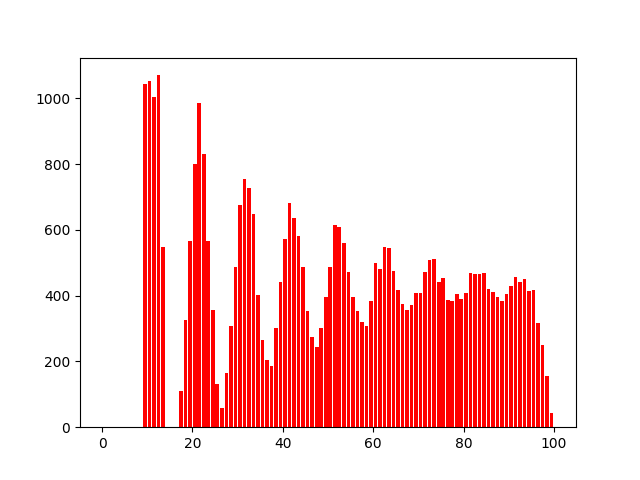
\includegraphics[width=0.8\textwidth]{Figure_1-1.png}
\end{center}
Above is the histogram for probability of collision 1. We see dark/dim spots. As the electrons starts accelerating from cathode it reaches critical velocity and the collides as p = 1 . And since velocity becomes zero it again starts accelerating reaches critical velocity and the process continues. These slowing down of electron results in dark spaces. Since continuously electrons are injected they will have a similar distribution and the overall intensity pattern will be superposition. Which results in these dark/dim spots.
\begin{center}
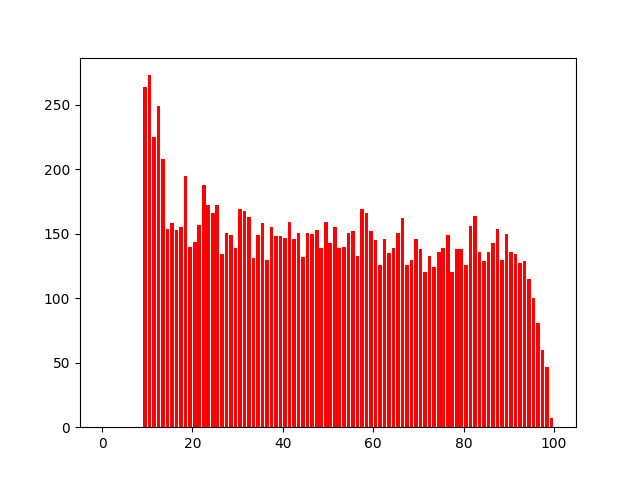
\includegraphics[width=0.8\textwidth]{Figure_1-2_5.png}
\end{center}
In case of probability 0.25 of collision the pattern followed is same as for probability 1. But minima's in the intensity is not visible because since the probability is 0.25 each curve spreads out and superposition of multiple of them ( from continuously injected electrons) give almost constant intensity after first electrons achieves critical velocity. A peak of intensity is observed and then it is almost constant.  
\begin{center}
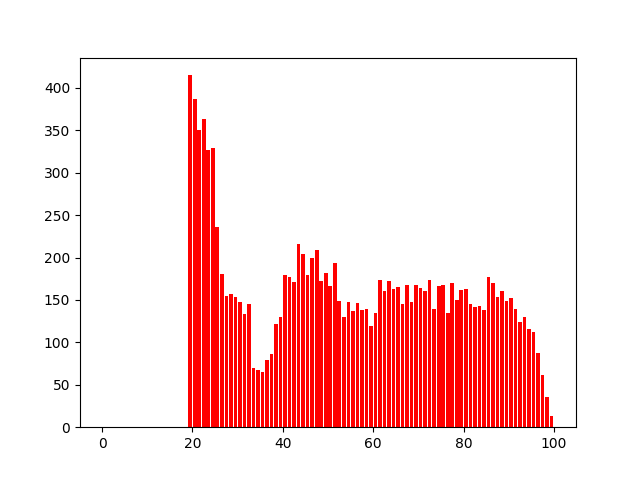
\includegraphics[width=0.8\textwidth]{Figure_1-v3.png}
\end{center}
The above histogram is for probability 0.5 and critical velocity 7 dim area after the peak is more significant. And from all the histogram , the nature of intensity variation can be well understood.
\begin{lstlisting}[language=Python]
plt.hist(I,bins=np.arange(0,101,1),rwidth=0.8,color = 'r')
plt.show()
\end{lstlisting}

\subsection{Histogram of Position}
\begin{center}
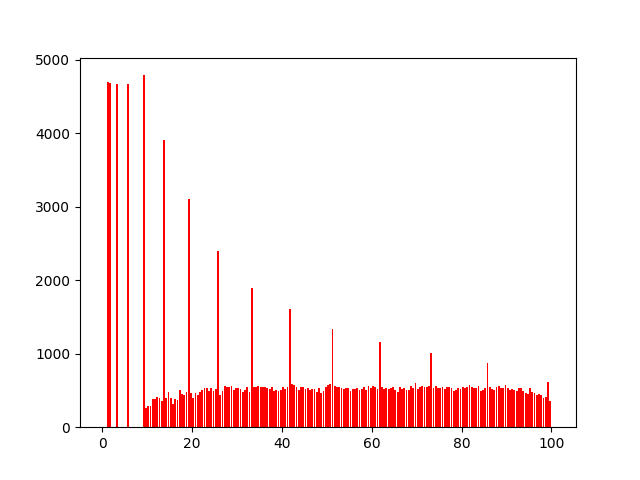
\includegraphics[width=0.8\textwidth]{Figure_2-v4.png}
\end{center}
The above histogram is calculated for critical velocity = 5, mean = 10, standard deviation = 2, bin width = 0.5.
The above histogram is for number of electron at a position in the tube. Before the position where electrons reach critical velocity the bars are of equal height and discrete gaps which shows uniformly accelerated electrons with no collisions. After collision the continuously decreasing peak (geometrically) which shows the fraction of each peak colliding. So the peak keeps of decreasing by the same fraction which should be equal to the probability of collision.
\begin{lstlisting}[language=Python]
plt.hist(X,bins=np.arange(0,101,1),rwidth=0.8,color = 'r')
plt.show()
\end{lstlisting}

\subsection{X vs V plot}
phase - space (position vs momentum) is represented by X  vs V. In this plot of X and V the outline (can be seen from equation of motion v$^{2}$ = u$^{2}$ + 2*a*x )  of the plot is tracing a parabola and the points inside the parabola are by the electrons colliding and loosing velocity. 
\begin{center}
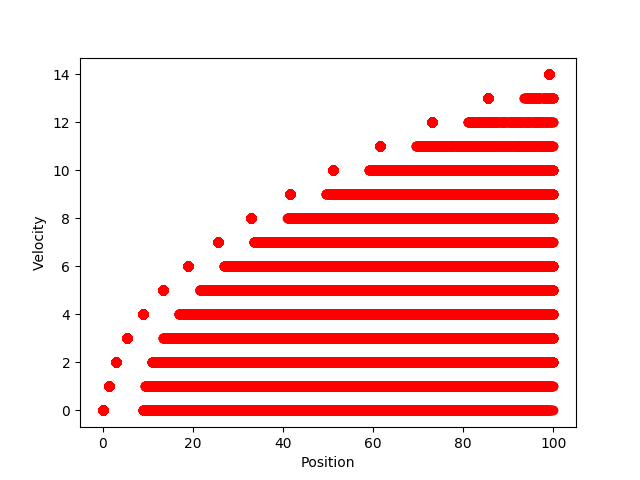
\includegraphics[width=0.8\textwidth]{Figure_3-2_5.png}
\end{center}
From 2-d histogram it is visible that the outline of the plot ( ones which did not collide ) have higher proportion which follows the parabola. (with p = 0.25)
\begin{center}
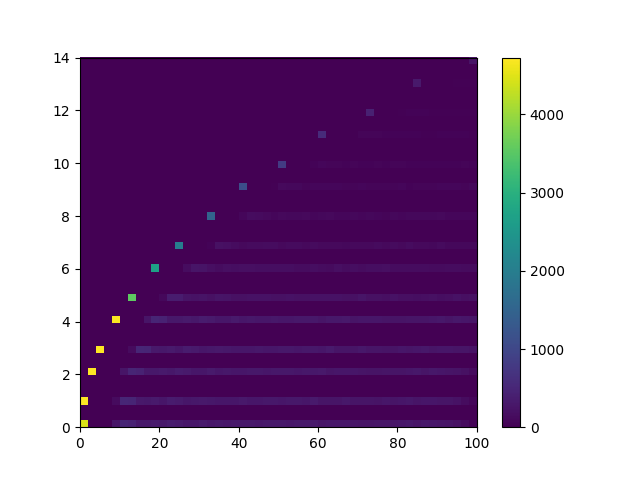
\includegraphics[width=0.8\textwidth]{Figure_4-2_5.png}
\end{center}
If we plot the same for p = 1 , the plot gets cut off at v =45 , as probability of collision is 1 and critical velocity is 5. So every electron reaching v = 5 will collide. 
\begin{center}
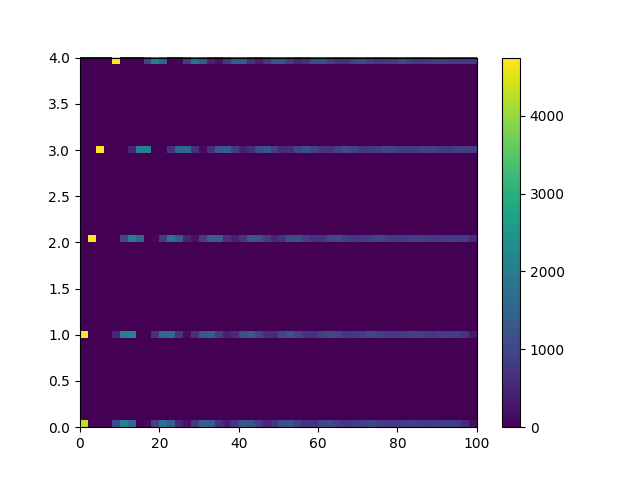
\includegraphics[width=0.8\textwidth]{Figure_4-1.png}
\end{center}
And for p = 0 , parabolic nature is followed perfectly.
\begin{center}
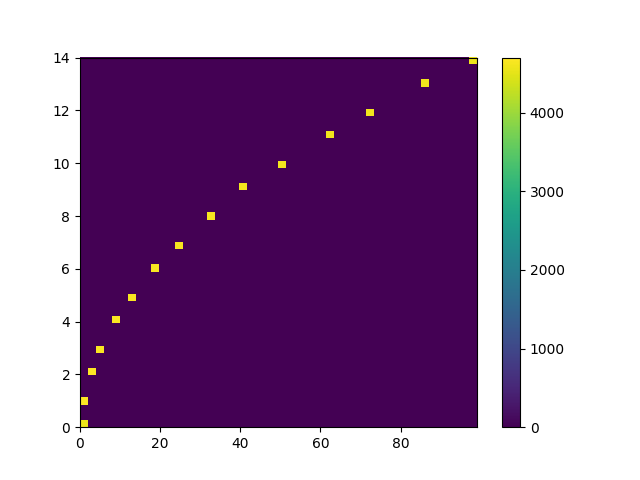
\includegraphics[width=0.8\textwidth]{Figure_4-0.png}
\end{center}
\begin{lstlisting}[language=Python]
#phase space of electron
plt.plot(X,V,'ro')
plt.xlabel("Position")
plt.ylabel("Velocity")
plt.show()

#plotting in 2-d histogram X,V
plt.hist2d(X,V,(50,50))
plt.colorbar()
plt.show()
\end{lstlisting}

\subsection{Intensity Data}
The table below shows the count of photons emitted from a particular position.
(for p = 0.25, mean = 10, critical velocity = 5 and standard deviation = 2)
\begin{lstlisting}[language=Python]
data = plt.hist(I,bins=np.arange(0,101,1),rwidth=0.8,color = 'r')
bins = data[1]
xpos = 0.5 * (bins[0:-1] + bins[1:])
df = pd.DataFrame({"xpos":xpos, "count":data[0]})
print tabulate(df, headers = 'keys', tablefmt = 'p' )
\end{lstlisting}
\subsection{Table of count of emitted photons vs position }
The table shows count of collision that is equal to the number of emitted photons vs position at which it emitted.
\verbatiminput{out.txt}
\section{Modification in existing model}
In the model used in this assignment assumes the than the collision between electron and atom happens between and random position between x$_{i}$ and x$_{i}$ + dx$_{i}$. The position between the between these position is selected by a uniformly distributed random number in position. From equation $$ v = u + \frac{1}{2}at^{2} $$
we can select uniformly distributed random number for time and substitute in equation to get position of collision. 
after colliding its velocity will become 0 and  it will again start accelerating till next time step (we are recording velocity an position at integer time steps). so we will update velocity as (1-dt) assuming unit acceleration and dt is random time instant when collision happened between one time step. Similarly position would be updated as, \textit{position of collision} + 0.5(1-dt)$^{2}$. 
\begin{lstlisting}[language=Python]
rho = np.random.rand(len(kl))# random time	
xx[kl] = ( xx[kl] - dx[kl] )  + ( u[kl] - 1 )*rho  + 0.5 * rho ** 2  	#finding exact position of collision between xi-1 and xi
xx[kl] =  x[kl] + (1 - rho) ** 2 #after colision velocity will be zero and it will aagain accelerate.
u[kl] = (1 - rho)	#making their velocity at after uniformly
\end{lstlisting}
plots obtained from this model are shown below
(for p = 0.25, mean = 10, standard deviation = 2, critical velocity = 5)
\begin{center}
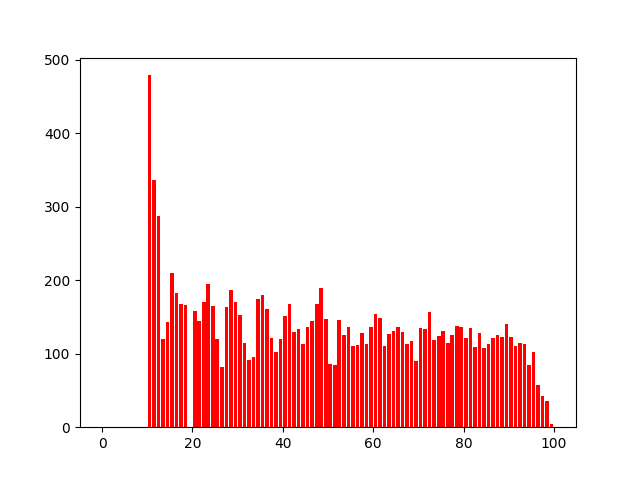
\includegraphics[width=0.8\textwidth]{Figure_1_v5.png}
\end{center}
\begin{center}
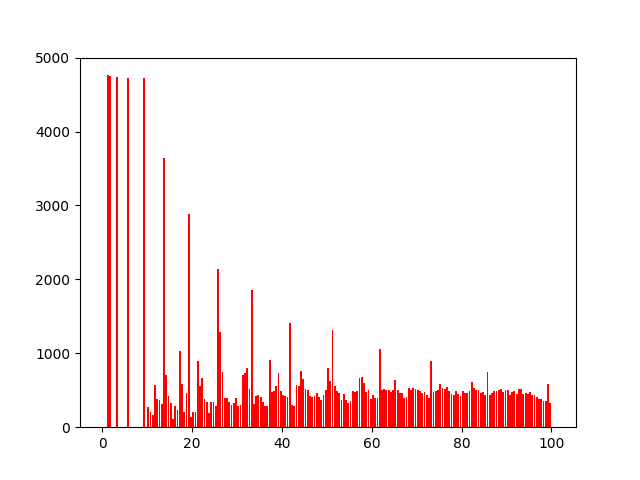
\includegraphics[width=0.8\textwidth]{Figure_2_v5.png}
\end{center}
\begin{center}
In the phase space plot velocity is no longer discretized . Continuous phase space in this model gives more accurate picture.
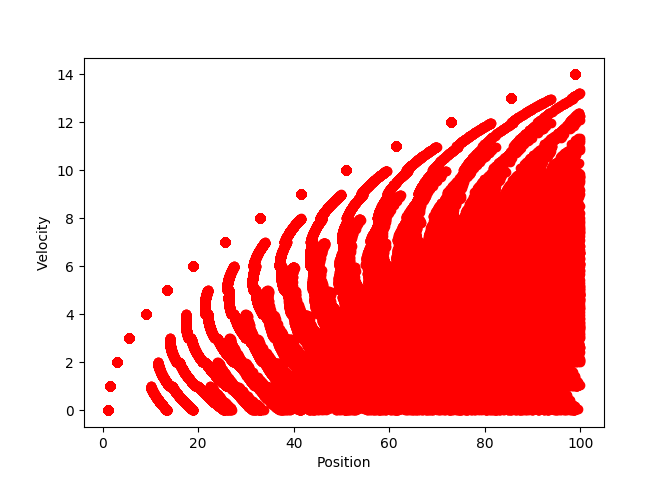
\includegraphics[width=0.8\textwidth]{Figure_3_v5.png}
\end{center}
\begin{center}
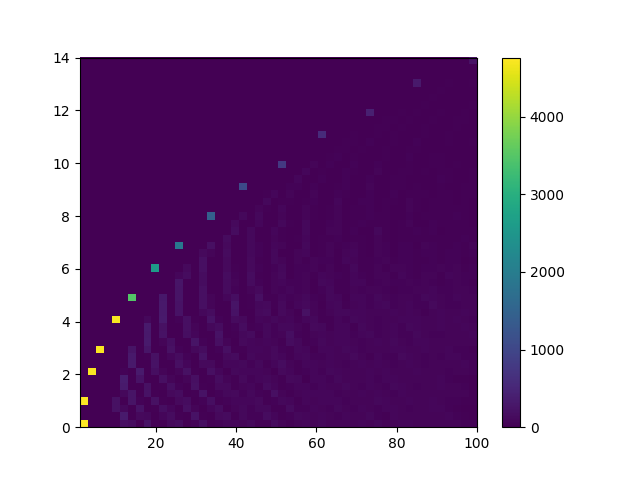
\includegraphics[width=0.8\textwidth]{Figure_4_v5.png}
\end{center}
\end{document}

